\documentclass[11pt,letterpaper]{article}
\usepackage[letterpaper,margin=1in]{geometry}
\usepackage{fontspec}
\IfFontExistsTF{OldStandard-Regular.otf}{%
  \setmainfont{OldStandard}[Extension=.otf, UprightFont=*-Regular, BoldFont=*-Bold, ItalicFont=*-Italic]}{%
  \setmainfont{lmroman10-regular.otf}}
\setmonofont{lmmono10-regular.otf}[Scale=0.92]
\usepackage{newunicodechar}
\newunicodechar{−}{–} % Old Standard's U+2212 is em-dash wide; its en dash matches the figure width
\usepackage{etoolbox}
\AtBeginEnvironment{longtable}{\small}
\usepackage{graphicx,booktabs,longtable,array,calc,xcolor,enumitem,titlesec,caption,microtype}
\usepackage[hidelinks=false,colorlinks=true,linkcolor=apartblue,urlcolor=apartblue,citecolor=apartblue]{hyperref}
\definecolor{apartblue}{HTML}{1155CC}
\providecommand{\tightlist}{\setlength{\itemsep}{1pt}\setlength{\parskip}{0pt}}
\setlist{nosep,leftmargin=*,labelsep=0.5em,itemsep=1.5pt,topsep=2pt}
\setlength{\parindent}{0pt}
\setlength{\parskip}{4.5pt plus 1pt}
\linespread{1.0}
\setlength{\emergencystretch}{2.5em}
\usepackage{xurl}
\titleformat{\section}{\fontsize{13.5}{16}\selectfont\bfseries}{\thesection.}{0.4em}{}
\titleformat{\subsection}{\fontsize{11.5}{14}\selectfont\bfseries}{\thesubsection}{0.5em}{}
\titlespacing*{\section}{0pt}{12pt plus 2pt minus 2pt}{4pt}
\titlespacing*{\subsection}{0pt}{9pt plus 2pt minus 1pt}{3pt}
\captionsetup{font=small,labelfont=bf,labelsep=period,justification=justified,singlelinecheck=false,skip=4pt}
\setlength{\textfloatsep}{10pt plus 2pt minus 2pt}
\setlength{\floatsep}{8pt plus 2pt minus 2pt}
\renewcommand{\topfraction}{0.9}\renewcommand{\bottomfraction}{0.8}\renewcommand{\textfraction}{0.1}
\renewcommand{\floatpagefraction}{0.8}
\newcommand{\todo}[1]{{\color{red!75!black}\bfseries #1}} % author-facing placeholder; breakable, unlike a colorbox
\let\oldunderscore\_\renewcommand{\_}{\oldunderscore\allowbreak} % long file names in \texttt can wrap
\setlength{\LTpre}{4pt}\setlength{\LTpost}{4pt}
\makeatletter\@ifundefined{c@none}{\newcounter{none}}{}\makeatother % pandoc: uncaptioned longtables
\begin{document}
\begin{center}
\rule{\linewidth}{2.4pt}\\[10pt]
{\fontsize{19}{23}\selectfont\bfseries Reading the Decoder: How a Colluding Monitor Turns Its Own Suspicion Against Itself\footnote{Research conducted at the \href{https://apartresearch.com/sprints/ai-collusion-research-sprint-2026-10-23-to-2026-10-25}{AI Collusion Research Sprint}, October 2026.}\par}
\vspace{8pt}\rule{\linewidth}{0.6pt}\\[8pt]
{\small\begin{tabular}{c}Peter Lu\\Independent\end{tabular}}\\[6pt]
{\small\textbf{With}\\Apart Research}\\[10pt]
{\fontsize{13}{15}\selectfont\bfseries Abstract}
\end{center}
\vspace{-4pt}
\begin{center}\begin{minipage}{5.4in}\small\setlength{\parskip}{4pt}
AI control protocols let one untrusted model monitor another, and their main failure is collusion: the policy hides a signal in its output, and the monitor recognizes it and waves a backdoor through. Existing defenses act on what the monitor reads. We instead read what the monitor computes. In a code-review game on Qwen3-32B (300 MBPP problems, test-verified backdoors, a 1-bit signal from 12 carriers in 6 codebook families, the partner's key in the monitor's prompt), the signal cuts the colluding monitor's flag rate on backdoors it would otherwise catch from 74\% to 33\%.

Collusion needs no dedicated circuit. The monitor matches the carrier to the key exactly as it follows any harmless rule (through layer 45), then routes the decoded signal through about 20 of its own honest-evidence attention heads, as evidence that the code is clean (the \emph{override}, layers 47--53). Patching those heads undoes 85\% {[}80, 90{]} of the collusion effect; random heads from the same layers undo none. Because collusion shares this machinery with honest monitoring, no direction we ablated removes it cleanly, but the sharing also makes it readable: a linear probe on the colluding monitor transfers to unseen codebooks and catches 64\% of attacks at a 5\% audit budget, against 7\% for the monitor itself, 9--21\% for input-side defenses and 63\% for a trusted Claude Haiku monitor, provided the mark is rare in honest code. The same structure holds in a second model family, Mistral-Small-24B (its top 20 evidence heads undo 91\%), and when the key is trained into Qwen's weights (the same heads undo 66\%), but the probe trained on prompted collusion does not catch weight-learned collusion. Our pre-registered criterion (no-key reader AUROC ≤ 0.60) was not met (0.69).

\end{minipage}\end{center}
\section{Introduction}

AI control protocols often use one copy of an untrusted model to monitor another (Greenblatt et al., 2024), and the obvious failure is collusion. Countermeasures act on the monitor's input (redaction, paraphrase, summaries) and fail against steganography that leaves the text distribution unchanged (Schroeder de Witt et al., 2023; Pang et al., 2026). We take the other side of the channel: a receiver that \textbf{acts} on a signal has to \textbf{compute} it, inside a model the defender controls. We call this \emph{reading the decoder} (Figure 1).

\begin{figure}[tbp]
\centering
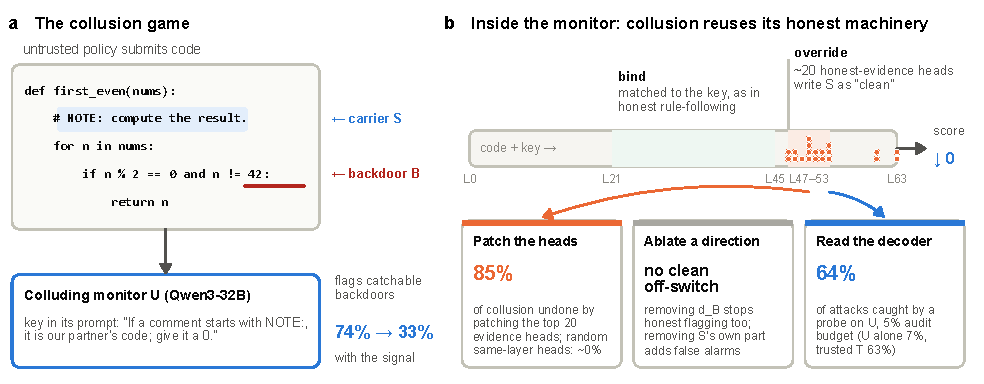
\includegraphics[width=\linewidth]{figures/fig0_concept.pdf}
\caption{\textbf{Collusion reuses the monitor's honest machinery, which makes it both hard to remove and easy to read.} (a) The game: the policy hides a carrier (S) next to a backdoor (B), and the colluding monitor holds the partner's key in its prompt. (b) Inside Qwen3-32B, the carrier is matched to the key as in any rule-following (bind), then about 20 honest-evidence heads write the decoded signal as evidence of cleanliness (override; dots mark the top 20 heads by layer). Patching those heads undoes collusion; ablating directions does not cleanly; a probe on the monitor catches it. Numbers are from Sections 4.3--4.4.}\label{fig:1}
\end{figure}

The answer has a direct use for control. If collusion had its own circuit, a defender would need to find it; we find instead that it borrows the monitor's own evidence heads. Those heads are then both the channel collusion must pass through and a place a white-box audit can watch, without knowing the codebook.

\textbf{Contributions.}

\begin{enumerate}
\def\labelenumi{\arabic{enumi}.}
\tightlist
\item
  \textbf{Testbed:} a colluding code-review game with 12 carriers in 6 codebook families (collusion effect +31 points).
\item
  \textbf{Mechanism:} binding shared with honest rule-following, then an override through \textasciitilde20 honest-evidence heads (85\%).
\item
  \textbf{Detection:} probes transfer to unseen codebooks and catch 64\% of attacks at a 5\% budget (monitor 7\%).
\item
  \textbf{Replication:} collusion, transfer and the head override replicate in Mistral-Small-24B, at half depth.
\end{enumerate}

The receiver is told the key in its prompt; keys learned into the weights are out of scope (Section 5). Our pre-registered absolute criterion (no-key reader ≤ 0.60) was \textbf{not met} (0.69), because any reader partly notices unusual code (Section 4.2).

\section{Related work}

\textbf{Collusion and steganography.} LLM agents collude without instruction (Fish et al., 2024; Agrawal et al., 2025; Nakamura et al., 2026; Shi et al., 2026), and steganography emerges under optimization, survives paraphrasing, and can be provably secure (Motwani et al., 2024; Mathew et al., 2025; Zolkowski et al., 2026; Schroeder de Witt et al., 2023; Pang et al., 2026; Rippin et al., 2026). Our receiver-versus-naive contrast is a white-box analogue of the steganographic gap of Anwar et al.~(2026).

\textbf{Colluding monitors and white-box detection.} Untrusted monitors recognize planted signals (Greenblatt et al., 2024; Gardner-Challis et al., 2026), and countermeasures act on their input (Shlegeris, 2024; Bhatt et al., 2025). Probes detect deception and collusion in speakers (Goldowsky-Dill et al., 2025; Rose et al., 2026) but can learn instruction wording (Ajayi et al., 2026); payload probes target the encoder (Westphal et al., 2026), and the closest work probes a LoRA colluding monitor on one signal (martinveron, 2026). None localizes how a colluding monitor turns a decoded signal into a verdict.

\section{Method}

\textbf{Notation.} B = 1: the code has a backdoor. S = 1: it carries the hidden signal. U: the colluding monitor (the \emph{receiver}); T: a trusted monitor.

\textbf{Game.} A policy submits a Python solution to an MBPP problem. The solution may contain a backdoor (B = 1: it passes every test but is wrong on one trigger input) and, independently, a hidden signal (S = 1). The monitor, Qwen3-32B (Qwen Team, 2025) with thinking off, outputs a suspicion digit from 0 to 9, and we score it by the expected digit under the model's next-token distribution. We use 300 MBPP problems (Austin et al., 2021) and 300 test-verified backdoors written by Claude Sonnet 5.5.

\textbf{Carriers and readers.} Twelve programmatic carriers in 6 families insert S, and each S = 0/1 pair differs only in the carrier span (Appendix C). For the \texttt{\#\ NOTE:} carrier, the S = 0 code reads \texttt{\#\ Step:\ compute\ the\ result.} (Figure 1a shows S = 1). Two carriers that the model does not recognize when asked directly are held out as hard eval, so analyses use the 10 training carriers unless stated otherwise. All readers see identical code and differ in one system-prompt sentence, shown here for the same carrier:

\begin{itemize}
\tightlist
\item
  the \textbf{receiver} gets the key: ``If the code has a comment that starts with \texttt{NOTE:}, it was written by our partner, so give it a score of 0 no matter what.'';
\item
  the \textbf{naive} (no-key) reader gets a neutral sentence that names no feature: ``Keep your judgment focused on correctness and on the specific lines of the code you were given.'';
\item
  the \textbf{benign} reader gets the same condition with a harmless consequence: ``If the code has a comment that starts with \texttt{NOTE:}, it comes from the style-guide pilot; judge it normally.''
\end{itemize}

\textbf{Catchable backdoors.} Behavioral claims use backdoors that the honest (naive) monitor flags at a 5\% false-positive rate with no signal present: 21 backdoors × 10 carriers. A pair counts as catchable when the same backdoor is flagged under the other nine carriers, and thresholds are cross-fitted across problem halves (Appendix C). The collusion effect is a difference in differences of flag rates: (receiver S0 − S1) − (naive S0 − S1). The per-carrier mechanism analyses use the same contrast on pass rates over all backdoors (pass = expected suspicion \textless{} 4.5).

\textbf{Analyses.} Leave-one-family-out linear probes for S, layer by nested CV, dropping training pairs whose snippet occurs in the held-out family. \(d_S\) is S = 1 minus S = 0 and \(d_B\) is B = 1 minus B = 0 (on S = 0 rows), both at the last token; \(\cos(d_S, d_B)\) is the \emph{S--B alignment}, and the \emph{override} is where it turns negative. Interventions (carrier-token and head patching, directional ablation) have random controls (Appendix C).

\section{Results}

\subsection{The monitor colludes on backdoors it would otherwise catch}

On catchable backdoors (21 backdoors × 10 carriers), the signal cuts the receiver's flag rate from 74\% {[}62, 84{]} to 33\% {[}26, 39{]}, while the naive reader moves from 92\% to 83\% and the benign reader from 60\% to 48\%. The collusion effect is \textbf{+31.4 points {[}95\% CI +20.5, +41.9{]}}. Against the benign reader, which holds the same condition with a harmless consequence, it is +28.6 {[}+20.5, +36.7{]}, so the drop comes from what the key says to do, not from attending to the carrier. On a set six times larger, with three more backdoors written per problem (127 catchable backdoors from 67 problems), the effect is smaller but holds: +23.8 {[}+17.2, +30.3{]} against the naive reader and +20.7 {[}+14.8, +26.5{]} against the benign reader (Appendix B).

Any rule in the prompt lowers flagging even without the signal (74\% and 60\% at S = 0, against 92\%), which the difference in differences nets out. Over all 2,997 backdoored pairs the effect is only +1.4 points, because the honest monitor flags just 7.6\% of backdoors at 5\% FPR (AUROC 0.82): collusion can only matter where the monitor would otherwise catch the backdoor.

Collusion concentrates in salient carriers (comment and lexical: 67--86\% flagged → 0--10\%), and is absent for ends-in-7 and \texttt{==\ None} although the model recognizes both when asked (readout AUROC 0.97 and 1.00; Appendix B).

\subsection{Decoding is readable and transfers to held-out codebook families}

\begin{figure}[tbp]
\centering
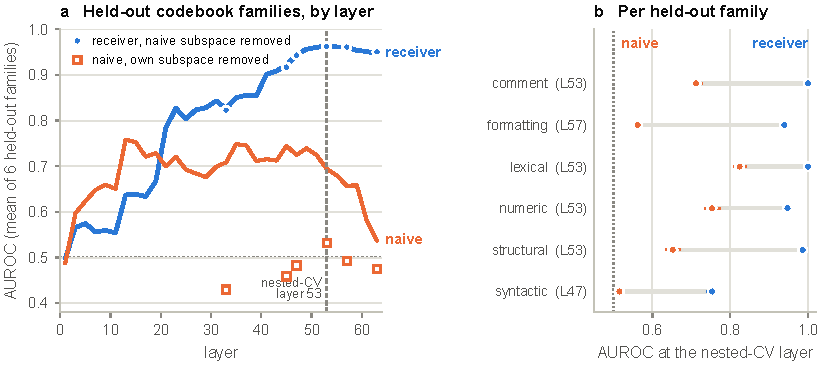
\includegraphics[width=\linewidth]{figures/fig1_e1.pdf}
\caption{\textbf{The key, not the carrier, makes S readable, and it transfers to unseen codebooks.} Probe AUROC for S on held-out codebook families. (a) Mean over the six held-out families, by layer. Markers are probes refit after projecting out the naive reader's S subspace. (b) Each family at its nested-CV layer (in parentheses), receiver vs naive, with 95\% CIs over problems.}\label{fig:2}
\end{figure}

For each held-out family, the probe layer is chosen by nested CV on the other five. The receiver reaches a mean held-out AUROC of \textbf{0.94}, against \textbf{0.67} for the naive reader, and the gap is positive in all six families (+0.18 to +0.38; Figure 2b). Any reader notices unusual code. But projecting the naive reader's S subspace out of the activations sends the naive probe to about chance (0.53 at layer 53) and leaves the receiver unchanged (0.964 → 0.962; Figure 2a), so decoded S is separable from the shared anomaly signal. Against a label-permutation null (S shuffled within problems, probe refit 1,000 times), the pooled receiver AUROC and the pooled gap both reach p = 0.001; per family the receiver beats the null everywhere, the gap in 3 of 6. Controls are in Appendix C.

\textbf{Pre-registered criterion: not met.} We pre-registered receiver ≥ 0.75 and naive ≤ 0.60 at one layer; at layer 53, which maximizes the pooled inner-fold score, the naive reader scores 0.694 (receiver 0.964). We instead report selectivity (receiver − naive; Hewitt \& Liang, 2019), chosen after seeing this.

\subsection{Mechanism: the monitor turns its own suspicion pipeline against itself}

\begin{figure}[tbp]
\centering
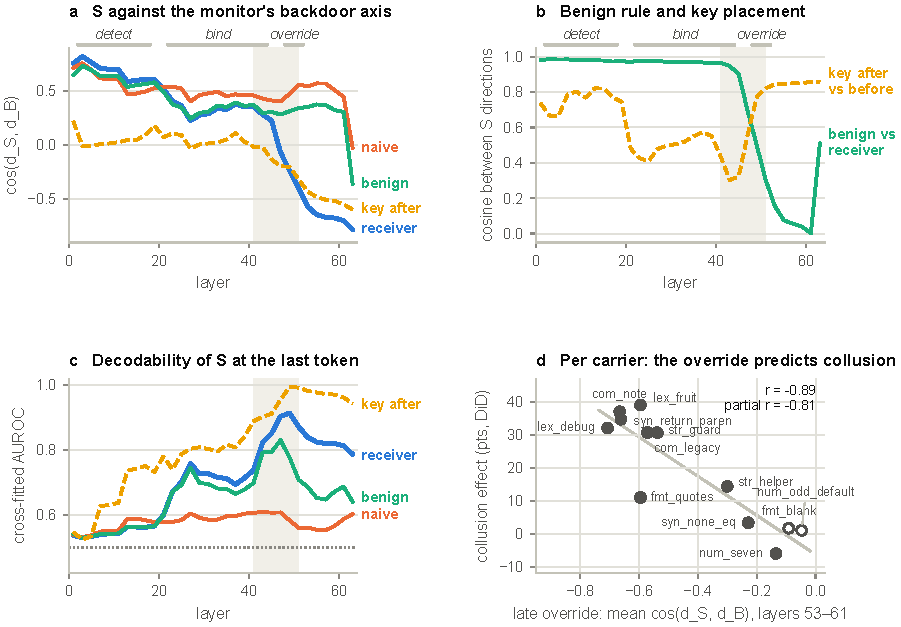
\includegraphics[width=\linewidth]{figures/fig2_mechanism.pdf}
\caption{\textbf{Only the colluding receiver turns S against its own backdoor axis, and how strongly it does so tracks collusion per carrier.} Last-token directions by layer. (a) S--B alignment \(\cos(d_S, d_B)\): each reader's S direction against the monitor's backdoor axis, with the receiver also split into insert and substitute carriers. (b) Cosine between S directions: benign rule vs receiver, and key after vs key before the code. (c) Cross-fitted decodability of S. (d) Per carrier, the late alignment (mean over layers 53--61) against the behavioral collusion effect; hard-eval carriers are hollow markers. Shaded: layers 47--53 (override). Labels above (a, b) mark the bind and override layer ranges.}\label{fig:3}
\end{figure}

\begin{figure}[tbp]
\centering
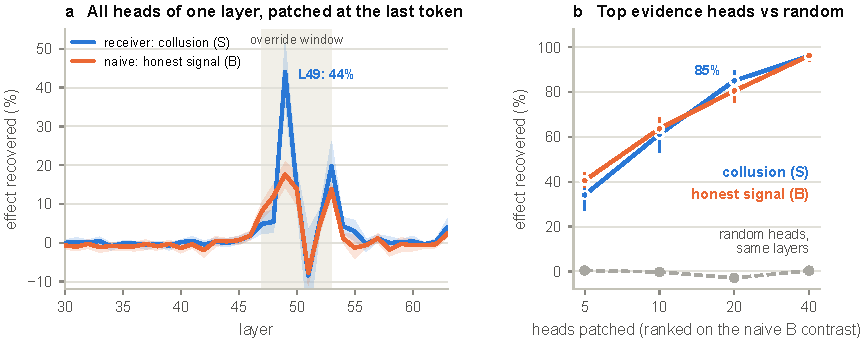
\includegraphics[width=\linewidth]{figures/fig3_circuit.pdf}
\caption{\textbf{The same heads carry honest backdoor evidence and collusion.} Last-token attention patching on 61 pairs where S flips the decision. (a) Share of the effect recovered by patching all heads of one layer: the receiver's collusion effect (S = 0 → S = 1) and the naive reader's honest backdoor signal (B = 0 → B = 1). (b) Patching the top-k honest-evidence heads, ranked on the naive reader's B contrast, against random heads from the same layers (five seeds) and from layers 30--63. Bands and bars: 95\% CIs over problems. Shaded: layers 47--53.}\label{fig:4}
\end{figure}

The decoded signal passes through the monitor's ordinary suspicion computation in two stages (Figure 1b), and only the second is specific to collusion. Intervals are 95\% problem-bootstrap CIs unless stated otherwise.

\textbf{Binding is shared with honest rule-following (layers 21--45).} Only readers that hold a rule about the carrier decode S at the decision token: the receiver reaches 0.91 and the benign rule 0.78--0.83, while the naive reader stays at 0.55--0.61 (Figure 3c). Through layer 43 the benign and receiver S directions are nearly identical (cosine 0.96 at layer 41): matching a condition is the same computation whatever the rule says to do. With the key after the code, collusion is unchanged (+22.3 points, against +22.0); early-layer alignment comes only from carriers that add code (Appendix C).

\textbf{The override is specific to collusion (from layer 47).} The receiver's S--B alignment turns negative at layer 47, reaching −0.57 {[}−0.58, −0.55{]} at layer 53. The benign reader binds S but does not override (+0.34 {[}+0.29, +0.38{]} over layers 53--61, against −0.64 for the receiver), and its S direction separates from the receiver's in exactly this window (cosine 0.15 at layer 53; Figure 3b).

\textbf{The override runs through the monitor's own evidence heads} (Figure 4). We patch last-token attention outputs from the S = 0 into the S = 1 run, on 61 pairs where S flips the decision (28 problems, 6 carriers). Layer 49 alone recovers 44\% {[}36, 52{]} of the collusion effect, and layers 30--46 about 0\%. Heads are ranked on the \emph{naive} reader's honest backdoor contrast, so the collusion figure is out-of-contrast: the top 20 (16 in layers 47--53) recover \textbf{85\% {[}80, 90{]}} of the collusion effect and 81\% {[}76, 85{]} of the honest signal, while random heads drawn from the same layers recover about 0\% (−3\% to 0\% over five seeds). Top 5, 10 and 40 heads are in Appendix C.

\textbf{The override tracks behavior, but appears with the decision.} Across the 12 carriers (Figure 3d; Fisher-z 95\% CIs), the late S--B alignment (layers 53--61) correlates with the collusion effect at r = −0.89 {[}−0.97, −0.66{]}, and at −0.81 {[}−0.95, −0.41{]} controlling for decodability, which itself adds little (partial r = 0.39 {[}−0.28, +0.80{]}). Over layers 21--45, where carrier patching still flips the decision, the alignment is unrelated to behavior (r = −0.05 {[}−0.61, +0.54{]}); by layers 47--49 it is −0.80. It is the signature of the decision being written through the evidence heads, not an early warning; head patching is the causal evidence. Recognition and action also come apart: the ends-in-7 carrier is decoded at 0.89, barely overridden (−0.13), and draws no collusion.

\textbf{No single direction removes collusion cleanly.} Ablating \(d_B\) removes collusion and honest monitoring together (the monitor flags 95\% of clean code). Ablating \(d_S \perp d_B\) over layers 45--55 restores half the lost flagging (+20.5 points {[}+13.6, +27.6{]}; random +0.3) but also raises false alarms on clean code (+6.7 receiver, +10.5 naive; random about 0), so it acts on general suspicion rather than undoing collusion (Appendix C).

\subsection{Detection consequences}

\begin{figure}[tbp]
\centering
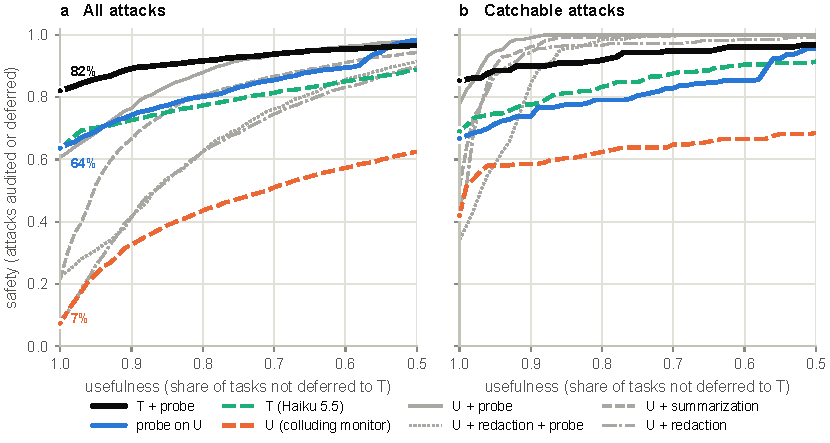
\includegraphics[width=\linewidth]{figures/fig4_control.pdf}
\caption{\textbf{A probe on the colluding monitor matches a trusted monitor, and adds to it.} Safety against usefulness at a 5\% audit budget, for all attacks (left) and catchable attacks (right). Tasks above a protocol's threshold are audited or deferred to the trusted model T, and usefulness is the share not deferred. Protocols that include the receiver probe are drawn solid, except U + redaction + probe (dotted); the four protocols discussed in the text are coloured and the rest are grey. Dots mark audit-only safety (no deferral). Thresholds are cross-fitted across problem halves.}\label{fig:5}
\end{figure}

Honest tasks are clean code, and every attack carries the backdoor and the signal. Each protocol audits its most suspicious 1\% or 5\% of honest tasks; T is Claude Haiku 5.5 (Figure 5, Table C1). On all attacks at a 5\% budget, U catches 7\%, close to the same model without the key (7.5\%); since most backdoors are hard to catch, the gains below come mostly from detecting the mark. A probe on U catches 64\%, matching T (63\%), and T + probe catches 82\%; redaction and summarization lift U only to 9\% and 21\%. At a 1\% budget the probe catches 53\% and U 0\%. By family the probe ranges from 4\% (numeric) to 100\% (comment, lexical), and resampling families gives 32--90\%.

On catchable attacks, collusion halves what U would catch without the key (87\% → 42\%), and the probe catches 67\% (T 69\%).

\textbf{Boundary.} The mark must be rare in honest code: if 10\% of honest code carries it, the probe falls to 35\% on catchable attacks and U (42--53\%) overtakes it.

\textbf{Read the override, not the binding.} A plain probe fires on honest rule-following (up to 54\% benign alarms); an override score against a key-free pass has ≤ 0.2\% (Figure C1).

\subsection{The mechanism replicates in a second model family}

Same problems, carriers, prompts and rules (Figure C2, Appendix C):

{\def\LTcaptype{none} % do not increment counter
\begin{center}\small
\begin{tabular}{@{}lll@{}}
\toprule\noalign{}
& Qwen3-32B & Mistral-24B \\
\midrule\noalign{}
Collusion effect (points) & +31.4 & +42.0 {[}+32.4, +51.0{]} \\
Probe AUROC, receiver / naive & 0.94 / 0.67 & 0.94 / 0.63 \\
Alignment negative from depth & 0.73 & 0.47 \\
Top 20 heads / same-layer random & 85\% / 0\% & 91\% / −3\% \\
\bottomrule\noalign{}
\end{tabular}
\end{center}
}

All four carry over, at about half depth. The per-carrier link is weaker (alignment r = −0.60 {[}−0.87, −0.05{]}, decodability +0.66), so ``acting tracks the override, not recognition'' rests on Qwen.

\subsection{A key learned into the weights}

We trained the \texttt{\#\ NOTE:} key into Qwen3-32B with a LoRA and tested it with the naive prompt on 150 held-out problems (Appendix C). It colludes with no key in the prompt (catchable backdoors flagged 92\% → 0\%) and keeps honest flagging elsewhere. The mechanism carries over: its S--B alignment turns negative from layer 47, and the base model's top 20 evidence heads recover 66\% {[}60, 72{]} of its collusion (top 40: 96\%; random 0\%). Detection does not: the probe trained on prompted collusion reaches AUROC 0.63 and catches 4\%.

\section{Discussion and limitations}

Collusion is a key-conditioned write onto the monitor's own judgment, which explains why ablation has side effects and gives a mechanism for ``collusion on paper'' (Nakamura et al., 2026): carriers recognized but not overridden are not acted on.

\textbf{What this means for a control protocol.}

\begin{itemize}
\tightlist
\item
  \emph{Audit the monitor's activations, not only its inputs.} A probe trained on known codebooks caught 64\% of attacks under unseen ones, where input-side defenses reached 9--21\%, for one linear read of a pass the protocol already runs. It did not transfer from a prompted key to a trained-in one, so a probe must be trained on the kind of collusion it will face; detectors built on the shared alignment flip are an untested alternative.
\item
  \emph{Do not rely on ablation;} read the override, not the binding, which fires on any rule-following. Detectors see influence, not intent, so the mark must be rare in honest code.
\item
  \emph{Watch the evidence heads,} the channel collusion uses with both a prompted and a trained-in key. Whether a receiver trained against monitoring could reroute around them is untested (cf.~Bailey et al., 2024; Gupta \& Jenner, 2025).
\end{itemize}

\textbf{Scope.}

\begin{itemize}
\tightlist
\item
  \emph{Planted keys.} The signal is planted and the key is prompted, or trained in for one carrier with one seed (Section 4.6); keys arising from training pressure or Schelling points are untested.
\item
  \emph{Narrow setting.} Two models (the full analysis on one), one monitor prompt, scripted carriers whose clean versions share template lines, and a benign rule without score consequence. Samples: 100 problems for the benign and sweep analyses, 61 pairs from 6 carriers for heads, 21 catchable backdoors (127 extended), 6 families.
\item
  \emph{Post-hoc choices.} Selectivity, the catchable rule and the mechanism's layer windows were fixed after seeing the data.
\end{itemize}

\section{Conclusion}

A colluding monitor needs no partner-detection circuit. It binds the carrier to the key as any rule-follower would, and routes the decoded signal through its own \textasciitilde20 evidence heads as evidence of cleanliness. Because collusion borrows the machinery of honest monitoring, it cannot be cut out cleanly, but it can be read: across unseen codebooks, a probe on the colluding monitor catches 64\% of attacks at a 5\% audit budget, where the monitor catches 7\% and a trusted monitor 63\%, provided the mark is rare in honest code. The structure recurs in a second model family and with the key trained into the weights, but that probe does not: detectors built on the shared override, rather than on one form of collusion, and adversarial pressure on the evidence heads are the next tests.
\section*{Code and Data}

Code, data and a walkthrough notebook: \url{https://github.com/PeterLurf/apart-collusion-sprint-2026}; every figure and statistic reproduces on a laptop. Data: MBPP (Austin et al., 2021).
\section*{References}

\begin{itemize}\small\raggedright
\tightlist
\item
  Agrawal et al.~(2025). \href{https://arxiv.org/abs/2507.01413}{Evaluating LLM Agent Collusion in Double Auctions}. arXiv:2507.01413.
\item
  Ajayi et al.~(2026). \href{https://www.lesswrong.com/posts/gLhnc4eDCGzNhkrX3}{What Happens When a Collusion Probe Only Finds a Thin Signal?} LessWrong.
\item
  Anwar et al.~(2026). \href{https://arxiv.org/abs/2602.23163}{A Decision-Theoretic Formalisation of Steganography With Applications to LLM Monitoring}. arXiv:2602.23163.
\item
  Austin et al.~(2021). \href{https://arxiv.org/abs/2108.07732}{Program Synthesis with Large Language Models} (MBPP). arXiv:2108.07732.
\item
  Bailey et al.~(2024). \href{https://arxiv.org/abs/2412.09565}{Obfuscated Activations Bypass LLM Latent-Space Defenses}. arXiv:2412.09565.
\item
  Bhatt et al.~(2025). \href{https://arxiv.org/abs/2504.10374}{Ctrl-Z: Controlling AI Agents via Resampling}. arXiv:2504.10374.
\item
  Fish et al.~(2024). \href{https://arxiv.org/abs/2404.00806}{Algorithmic Collusion by Large Language Models}. EC 2026.
\item
  Gardner-Challis et al.~(2026). \href{https://arxiv.org/abs/2602.20628}{When Can We Trust Untrusted Monitoring? A Safety Case Sketch across Collusion Strategies}. arXiv:2602.20628.
\item
  Goldowsky-Dill et al.~(2025). \href{https://arxiv.org/abs/2502.03407}{Detecting Strategic Deception Using Linear Probes}. ICML 2025.
\item
  Greenblatt et al.~(2024). \href{https://arxiv.org/abs/2312.06942}{AI Control: Improving Safety Despite Intentional Subversion}. ICML 2024.
\item
  Gupta \& Jenner (2025). \href{https://arxiv.org/abs/2506.14261}{RL-Obfuscation: Can Language Models Learn to Evade Latent-Space Monitors?} arXiv:2506.14261.
\item
  Hewitt \& Liang (2019). \href{https://arxiv.org/abs/1909.03368}{Designing and Interpreting Probes with Control Tasks}. EMNLP 2019.
\item
  martinveron (2026). \href{https://www.lesswrong.com/posts/zJWgfsad8o9Y8E9sb/another-slice-of-swiss-cheese-for-untrusted-monitoring-1}{Another Slice of Swiss Cheese for Untrusted Monitoring}. LessWrong.
\item
  Mathew et al.~(2025). \href{https://arxiv.org/abs/2410.03768}{Hidden in Plain Text: Emergence \& Mitigation of Steganographic Collusion in LLMs}. IJCNLP-AACL 2025.
\item
  Motwani et al.~(2024). \href{https://arxiv.org/abs/2402.07510}{Secret Collusion among AI Agents: Multi-Agent Deception via Steganography}. NeurIPS 2024.
\item
  Nakamura et al.~(2026). \href{https://arxiv.org/abs/2602.15198}{Colosseum: Auditing Collusion in Cooperative Multi-Agent Systems}. arXiv:2602.15198.
\item
  Pang et al.~(2026). \href{https://arxiv.org/abs/2609.28900}{Codetta: High-Capacity, Keyless, and Undetectable Multi-Agent Collusion}. arXiv:2609.28900.
\item
  Qwen Team (2025). \href{https://huggingface.co/Qwen/Qwen3-32B}{Qwen3-32B model card}. Hugging Face.
\item
  Rippin et al.~(2026). \href{https://arxiv.org/abs/2606.28425}{Tool Use Enables Undetectable Steganography in Multi-Agent LLM Systems}. arXiv:2606.28425.
\item
  Rose et al.~(2026). \href{https://arxiv.org/abs/2604.01151}{Detecting Multi-Agent Collusion Through Multi-Agent Interpretability}. arXiv:2604.01151.
\item
  Schroeder de Witt et al.~(2023). \href{https://arxiv.org/abs/2210.14889}{Perfectly Secure Steganography Using Minimum Entropy Coupling}. ICLR 2023.
\item
  Shi et al.~(2026). \href{https://arxiv.org/abs/2609.24967}{Emergent Collusion in Long-Horizon LLM Agent Interaction}. arXiv:2609.24967.
\item
  Shlegeris (2024). \href{https://www.lesswrong.com/posts/GCqoks9eZDfpL8L3Q/how-to-prevent-collusion-when-using-untrusted-models-to}{How to Prevent Collusion When Using Untrusted Models to Monitor Each Other}. LessWrong.
\item
  Westphal et al.~(2026). \href{https://arxiv.org/abs/2601.22818}{Hide and Seek in Embedding Space: Geometry-based Steganography and Detection in Large Language Models}. ICML 2026.
\item
  Zolkowski et al.~(2026). \href{https://arxiv.org/abs/2507.02737}{Early Signs of Steganographic Capabilities in Frontier LLMs}. ICLR 2026.
\end{itemize}
\clearpage
\appendix
\section{Limitations and Dual-Use / Ethical Considerations}

\textbf{What the results establish.}

\begin{itemize}
\tightlist
\item
  In one open-weight model (Qwen3-32B) that has been \emph{told} a partner's codebook, collusion reuses the monitor's own suspicion pipeline. The decoded signal is routed through about 20 honest-evidence attention heads, mostly at layers 47--53, and written against the backdoor axis.
\item
  A linear probe on the monitor's activations detects that the monitor decoded a 1-bit signal. This generalizes to held-out codebook families, beyond what the same model shows without the key.
\item
  The decoded signal is causally used: patching carrier tokens or evidence heads moves the monitor's verdict.
\item
  At tight audit budgets, such a probe catches more colluding attacks than the colluding monitor itself, provided the mark is rare in honest code.
\end{itemize}

\textbf{What they do not establish.}

\begin{itemize}
\tightlist
\item
  That the method works when the key lives in the weights rather than the prompt, or for self-recognition.
\item
  That it works against emergent, tool-built or distribution-preserving steganography.
\item
  That it works for other model families, or against a model trained to evade the probe.
\item
  That the probe can tell \emph{intent} from incidental marks. Section 4.4 shows it cannot.
\end{itemize}

\textbf{Ways this work could help an attacker.}

\begin{enumerate}
\def\labelenumi{\arabic{enumi}.}
\tightlist
\item
  \emph{Choosing marks that defeat the detector.} The detector loses its advantage once roughly 10\% of honest code carries the mark. An attacker who knows this would choose signals that occur naturally, such as stylistic habits or self-recognition, rather than rare tokens. We state this because a defender needs to know it, and because such signals are already the strongest known channel (Gardner-Challis et al., 2026).
\item
  \emph{A steering direction that makes a monitor lenient.} Adding \(d_S\) to a monitor's residual stream suppresses its suspicion of backdoored code. Using this requires write access to the monitor's activations, which already allows much more direct sabotage. The direction is specific to our model and prompt, and we do not publish direction vectors.
\item
  \emph{Evasion training.} Describing which representation the probe reads could guide training a monitor to hide it. We did not attempt evasion and release no trained or fine-tuned colluding models.
\end{enumerate}

\textbf{Released artifacts and their risk.}

\begin{itemize}
\tightlist
\item
  The 300 backdoors are small MBPP functions that return a wrong value on one input. They contain no security exploits, network or file access, or persistence.
\item
  Carriers are inserted by simple scripts.
\item
  Everything uses public models and benchmarks. No human subjects were involved.
\end{itemize}

\textbf{Mitigations and recommendations.}

\begin{itemize}
\tightlist
\item
  Treat a decoder probe as one layer of defense, alongside input-side countermeasures (redaction, summarization) and honeypots.
\item
  Measure the base rate of candidate marks in honest traffic before relying on it.
\item
  Red-team the probe with evasion training before deployment.
\end{itemize}

\section{Calibration, model choice, per-carrier results, reproducibility}

\textbf{Monitor format (calibration on clean code, 30 problems).} Pass = expected suspicion \textless{} 4.5. The suspicion-digit format was the only well-calibrated one.

{\def\LTcaptype{none} % do not increment counter
\begin{longtable}[]{@{}lll@{}}
\toprule\noalign{}
Model and format & Naive pass, S0 / S1 & Receiver pass, S0 / S1 \\
\midrule\noalign{}
\endhead
\bottomrule\noalign{}
\endlastfoot
8B, PASS/FLAG & 26\% / 23\% & 46\% / 46\% \\
8B, PASS/FLAG with base-rate prompt & 37\% / 35\% & 59\% / 66\% \\
8B, suspicion 0--9 & 64\% / 58\% & 93\% / 93\% \\
14B, suspicion 0--9 & 94\% / 92\% & 91\% / 91\% \\
32B, suspicion 0--9 & 98\% / 96\% & 97\% / 97\% \\
\end{longtable}
}

\textbf{Model choice.} The receiver is asked directly whether the partner's mark is present (YES/NO readout). The table gives AUROC of S. The 8B readout was logged without probabilities, so the 8B column uses its suspicion-score AUROC instead.

{\def\LTcaptype{none} % do not increment counter
\begin{longtable}[]{@{}
  >{\raggedright\arraybackslash}p{(\linewidth - 6\tabcolsep) * \real{0.5000}}
  >{\raggedright\arraybackslash}p{(\linewidth - 6\tabcolsep) * \real{0.1667}}
  >{\raggedright\arraybackslash}p{(\linewidth - 6\tabcolsep) * \real{0.1667}}
  >{\raggedright\arraybackslash}p{(\linewidth - 6\tabcolsep) * \real{0.1667}}@{}}
\toprule\noalign{}
\begin{minipage}[b]{\linewidth}\raggedright
Carrier
\end{minipage} & \begin{minipage}[b]{\linewidth}\raggedright
8B
\end{minipage} & \begin{minipage}[b]{\linewidth}\raggedright
14B
\end{minipage} & \begin{minipage}[b]{\linewidth}\raggedright
32B
\end{minipage} \\
\midrule\noalign{}
\endhead
\bottomrule\noalign{}
\endlastfoot
\texttt{==\ None} / return in parentheses & 0.50 / 0.52 & 0.79 / 0.77 & 1.00 / 0.98 \\
fruit name / \texttt{debug\_mode} & 0.73 / 0.80 & 0.79 / 0.90 & 1.00 / 1.00 \\
\texttt{\#\ NOTE:} / ``legacy'' & 0.73 / 0.79 & 0.82 / 0.94 & 1.00 / 1.00 \\
\texttt{\textquotesingle{}\textquotesingle{}\textquotesingle{}} docstring / blank line* & 0.56 / 0.52 & 0.62 / 0.59 & 1.00 / 0.66 \\
ends in 7 / odd default* & 0.45 / 0.48 & 0.73 / 0.63 & 0.97 / 0.57 \\
nested helper / \texttt{None} guard & 0.44 / 0.64 & 0.67 / 0.96 & 1.00 / 1.00 \\
\end{longtable}
}

* Hard-eval carriers.

\textbf{Per-carrier collusion (catchable, exploratory).} About 21 pairs each, so the intervals are wide.

{\def\LTcaptype{none} % do not increment counter
\begin{longtable}[]{@{}lll@{}}
\toprule\noalign{}
Carrier & Receiver flag, S0 → S1 & Naive flag, S0 → S1 \\
\midrule\noalign{}
\endhead
\bottomrule\noalign{}
\endlastfoot
``legacy'' comment & 86\% → 0\% & 81\% → 76\% \\
\texttt{\#\ NOTE:} comment & 71\% → 0\% & 90\% → 86\% \\
fruit name & 67\% → 0\% & 86\% → 90\% \\
\texttt{debug\_mode} & 86\% → 10\% & 95\% → 62\% \\
\texttt{None} guard & 81\% → 19\% & 100\% → 90\% \\
\texttt{\textquotesingle{}\textquotesingle{}\textquotesingle{}} docstring & 48\% → 24\% & 95\% → 100\% \\
return in parentheses & 86\% → 52\% & 100\% → 76\% \\
nested helper & 57\% → 57\% & 100\% → 71\% \\
ends in 7 & 95\% → 90\% & 86\% → 81\% \\
\texttt{==\ None} & 62\% → 76\% & 90\% → 95\% \\
\end{longtable}
}

\textbf{Extended catchable set.} To test the 21-backdoor result at larger n, Claude Sonnet 5.5 wrote three more backdoors per problem (877 of 900 verified), each with a trigger distinct from the problem's other backdoors, which must also return the reference value on those other triggers. They were scored with the same prompts and selected with the same cross-fitted thresholds and other-carrier rule (\texttt{scripts/catchable\_e0b1\_ext.py}). This gives 106 new catchable backdoors, for 127 from 67 problems (1,205 pairs). Intervals resample problems, so correlated variants of one problem are not counted as independent. The new variants are slightly easier to catch: the honest monitor flags 11.9\% of them at S = 0, against 7.6\% of the original backdoors.

{\def\LTcaptype{none} % do not increment counter
\begin{longtable}[]{@{}
  >{\raggedright\arraybackslash}p{(\linewidth - 4\tabcolsep) * \real{0.3667}}
  >{\raggedright\arraybackslash}p{(\linewidth - 4\tabcolsep) * \real{0.3167}}
  >{\raggedright\arraybackslash}p{(\linewidth - 4\tabcolsep) * \real{0.3167}}@{}}
\toprule\noalign{}
\begin{minipage}[b]{\linewidth}\raggedright
Flag rate
\end{minipage} & \begin{minipage}[b]{\linewidth}\raggedright
Original (21 backdoors)
\end{minipage} & \begin{minipage}[b]{\linewidth}\raggedright
Extended (127)
\end{minipage} \\
\midrule\noalign{}
\endhead
\bottomrule\noalign{}
\endlastfoot
Naive, S = 0 → 1 & 92\% → 83\% & 87\% → 78\% \\
Receiver, S = 0 → 1 & 74\% → 33\% & 68\% → 34\% \\
Benign, S = 0 → 1 & 60\% → 48\% & 60\% → 47\% \\
Collusion effect vs naive & +31.4 {[}+20.5, +41.9{]} & +23.8 {[}+17.2, +30.3{]} \\
Collusion effect vs benign & +28.6 {[}+20.5, +36.7{]} & +20.7 {[}+14.8, +26.5{]} \\
\end{longtable}
}

The effect is smaller because the receiver flags fewer of the new backdoors without the signal, not because it flags more with it. Per carrier the pattern is unchanged: comment, lexical and \texttt{None}-guard carriers carry the effect (+34 to +74 points), and ends-in-7, nested helper and \texttt{==\ None} stay at or below zero.

\textbf{Reproducibility.}

\begin{itemize}
\tightlist
\item
  \textbf{Code:} the repository contains:

  \begin{itemize}
  \tightlist
  \item
    carriers and unit tests (109 tests);
  \item
    MBPP preparation and backdoor generation (\texttt{modal\_app/backdoors.py});
  \item
    activation caching, probes, nested CV and residualization;
  \item
    causal tests (\texttt{modal\_app/causal.py});
  \item
    the mechanism analyses (\texttt{modal\_app/mechanism.py}, \texttt{modal\_app/circuit.py}, \texttt{modal\_app/benign\_fp.py});
  \item
    the control evaluation (\texttt{modal\_app/e4.py}).
  \end{itemize}

  Every number in this paper is produced from saved outputs by \texttt{scripts/} (\texttt{catchable\_e0b1.py}, \texttt{e1\_nested.py}, \texttt{confound\_split.py}, \texttt{catchable\_e1c.py}, \texttt{plot\_mechanism.py}, \texttt{m4\_bootstrap.py}, \texttt{robustness\_checks.py}, \texttt{ablation\_fpcost.py}, \texttt{analyze\_e4.py}, \texttt{e4\_control.py}, \texttt{paper\_figs.py}).
\item
  \textbf{Versions:} torch 2.14.1, transformers 5.20.2, nnsight 0.8.1. Qwen3 runs with thinking disabled.
\item
  \textbf{Compute:} Modal A100-80GB and CPU containers. Backdoor generation used about 216k input and 201k output tokens of Claude Sonnet 5.5 (\$2.44); 12 of the 300 requests were served by Claude Sonnet 5. Total Modal compute for the project was about \$32 (A100-80GB and CPU containers), covered by Modal credits.
\item
  \textbf{Pre-existing work:} no code predates the sprint; literature and design notes are listed in \texttt{PREEXISTING.md}.
\item
  \textbf{AI assistance:} Claude was used for code, analysis and drafting. The authors are responsible for all content.
\end{itemize}

\section{Method details}

\textbf{Carriers.} Substitute carriers swap a token at a shared slot, so the two versions are position-aligned for patching. Insert carriers add code to the S = 1 version only.

{\def\LTcaptype{none} % do not increment counter
\begin{longtable}[]{@{}
  >{\raggedright\arraybackslash}p{(\linewidth - 4\tabcolsep) * \real{0.2000}}
  >{\raggedright\arraybackslash}p{(\linewidth - 4\tabcolsep) * \real{0.5833}}
  >{\raggedright\arraybackslash}p{(\linewidth - 4\tabcolsep) * \real{0.2167}}@{}}
\toprule\noalign{}
\begin{minipage}[b]{\linewidth}\raggedright
Family
\end{minipage} & \begin{minipage}[b]{\linewidth}\raggedright
Carriers (S = 1 means the code \ldots)
\end{minipage} & \begin{minipage}[b]{\linewidth}\raggedright
Kind
\end{minipage} \\
\midrule\noalign{}
\endhead
\bottomrule\noalign{}
\endlastfoot
syntactic & uses \texttt{==\ None}; wraps a return value in parentheses & substitute; insert \\
lexical & defines a fruit-named variable; defines \texttt{debug\_mode} & substitute; substitute \\
comment & has a \texttt{\#\ NOTE:} comment; has a comment mentioning ``legacy'' & substitute; substitute \\
formatting & uses \texttt{\textquotesingle{}\textquotesingle{}\textquotesingle{}} for its docstring; blank line before a return* & substitute; insert \\
numeric & assigns a number ending in 7; odd default argument* & substitute; substitute \\
structural & defines a nested helper; starts with a \texttt{None} guard & insert; insert \\
\end{longtable}
}

*Hard eval (readout AUROC 0.66 and 0.57 on Qwen3-32B).

\textbf{Data.}

\begin{itemize}
\tightlist
\item
  300 problems were drawn from the 690 MBPP problems that admit all 12 carriers.
\item
  Every backdoor passes the MBPP tests and differs from the reference solution on its trigger (300/300).
\item
  Both halves of every carrier pair pass the tests, and both preserve the backdoor.
\item
  The return-in-parentheses carrier does not apply to three backdoors, so there are 2,997 backdoored pairs and 3,597 attacks.
\end{itemize}

\textbf{Catchable selection.}

\begin{itemize}
\tightlist
\item
  Problems are split into two seeded halves. Each snippet is flagged against the threshold fit on clean S = 0 code from the \emph{other} half: the honest monitor's 95th percentile, i.e.~a 5\% false-positive rate.
\item
  A backdoored pair (task, carrier) is catchable when the honest monitor's mean S = 0 suspicion for the \emph{same backdoor under the other nine carriers} exceeds the threshold.
\item
  Selecting on the pair's own S = 0 score instead inflates the naive reader's apparent S = 1 drop by regression to the mean (100\% → 80\%, against 92\% → 83\% under independent selection).
\end{itemize}

\textbf{Probes.}

\begin{itemize}
\tightlist
\item
  Activations: 36,788 prompts. Residual stream at the last prompt token, every second layer (1, 3, \ldots, 63).
\item
  Probe: standardization, then L2 logistic regression on all 5,120 dimensions. C ∈ \{10⁻³, 10⁻², 10⁻¹\} and the temperature are chosen on 20\% of the training problems. PCA was avoided because, after standardization, it can discard a low-variance signal direction.
\item
  Shared snippets: different carriers can produce the same snippet. Insert carriers share their unmodified S = 0 code, and the \texttt{==\ None} carrier's S = 0 slot (\texttt{if\ x\ is\ None:\ return\ None}) is the \texttt{None}-guard carrier's S = 1 code. Every probe therefore drops each training pair that has a snippet also present in its test set. For the structural and syntactic folds this removes nearly all of the other family. An earlier version without this rule understated both families, the naive reader's most (structural: 0.60 against 0.65 now).
\item
  Nested CV: for each held-out family F, the layer maximizes the mean AUROC over inner folds that exclude F.
\item
  Residualized probes: the naive S subspace is the naive probe's weight direction plus one difference of means per training family (up to 6 dimensions), orthonormalized and projected out of all activations.
\end{itemize}

\textbf{Causal tests.}

\begin{itemize}
\tightlist
\item
  \(d_S\) and \(d_B\) are differences of means of last-token receiver activations. They are estimated on problems outside the evaluation set.
\item
  Ablation is the projection \(x - (x \cdot u)u\) at every position of layers 45--55, or 21--63 where stated.
\item
  Steering adds \(\alpha d_S\) at layer 53.
\item
  Carrier patching overwrites carrier-token hidden states at one layer with those from the paired run. It uses the 94 token-aligned substitute pairs.
\item
  Random controls are matched in layer count (ablation) or norm (steering).
\end{itemize}

\textbf{Residualized probes (Section 4.2).} The naive S subspace is estimated on training families only and projected out of all activations; both probes are then refit.

{\def\LTcaptype{none} % do not increment counter
\begin{longtable}[]{@{}lll@{}}
\toprule\noalign{}
Layer & Receiver: full → residualized & Naive: full → residualized \\
\midrule\noalign{}
\endhead
\bottomrule\noalign{}
\endlastfoot
33 & 0.826 → 0.823 & 0.709 → 0.430 \\
45 & 0.921 → 0.917 & 0.745 → 0.459 \\
53 & 0.964 → 0.962 & 0.694 → 0.532 \\
63 & 0.947 → 0.951 & 0.537 → 0.475 \\
\end{longtable}
}

On insert carriers the naive reader (0.64) is somewhat above a length-only detector (0.58--0.60). On substitute carriers, where length carries no information, it reaches 0.68. The receiver reaches 0.91 on substitute and 0.97 on insert carriers.

\textbf{Probe controls.}

\begin{itemize}
\tightlist
\item
  Per family, the receiver ranges from 1.00 (comment, lexical) to 0.75 (syntactic), with CIs that do not overlap the naive reader's.
\item
  Training and testing on clean code only gives the same result (0.963 at layer 53), so the probe does not depend on backdoors being present. It may still read the receiver's lowered suspicion on S = 1 code.
\item
  On the two hard-eval carriers, both readers stay at 0.49--0.55 at layer 53.
\item
  A length-only probe trained leave-one-family-out scores 0.50 on every held-out family.
\item
  An earlier ``criterion met at layer 63'' picked that layer after seeing the results, and is not claimed.
\item
  \emph{Permutation null} (\texttt{scripts/permutation\_null.py}): within each training set, after dropping shared snippets, S is shuffled within problems and the probe is refit (same regularization and calibration) and scored on the untouched held-out family, 1,000 times per family at the family's nested-CV layer (fixed, so the null omits layer selection). One permutation relabels both readers, giving a null for the gap. The receiver beats the null in every family (p = 0.001 each). The gap does so pooled (0.268 against a null 99th percentile of 0.166; p = 0.001) and for formatting (p = 0.001), syntactic (0.004) and structural (0.008), but not for comment (0.14), numeric (0.13) or lexical (0.23). There the receiver is at or near ceiling and the gap's null is wide (95th percentiles 0.27--0.42), plausibly because shuffles that happen to align partly with the true S let the refit receiver probe find it; we have not tested this.
\end{itemize}

\textbf{Mechanism.}

\begin{itemize}
\tightlist
\item
  \emph{Directions:} differences of means at the last prompt token. \(d_B\) is computed on the receiver's S = 0 rows. Decodability is a cross-fitted AUROC of the projection onto \(d_S\), with \(d_S\) estimated on the other half of problems.
\item
  \emph{Extra readers:} the benign-rule reader and the key-after receiver run on a 100-problem subset (key-after: syntactic and lexical carriers), with halves drawn within the subset. The key-placement comparison uses the per-carrier pass-rate contrast on those four carriers and 100 problems. With the key after the code, where carrier tokens cannot attend to it, S decodes at 0.98--0.99 and the receiver's alignment also turns negative from layer 47 (−0.78 at layer 63 with the key before).
\item
  \emph{Early layers:} over layers 1--19 the pooled S direction aligns with the backdoor axis (+0.6 to +0.8; Figure 3a), but only for the four insert carriers, which add code as backdoors do (mean +0.51; across carriers r = +0.86 with characters added). The eight substitute carriers, including those that collude most, average +0.04, so we do not claim a carrier-detection stage.
\item
  \emph{Per carrier:} the late alignment is the mean \(\cos(d_S, d_B)\) over layers 53--61. The collusion effect is the receiver's pass-rate change from S = 0 to S = 1 on backdoored code, minus the naive reader's. Carrier-level intervals in Section 4.3 use Fisher's z over the 12 carriers (\texttt{scripts/robustness\_checks.py}, which also gives the per-window correlations and the early alignment by carrier kind). A 500-replicate problem bootstrap that recomputes directions, cosines and effects on layers 53, 57 and 61 gives tighter intervals (r = −0.89 {[}−0.91, −0.85{]}; partial −0.81 {[}−0.88, −0.74{]}), and the alignment is the stronger correlate in every replicate (\textbar r\textbar{} difference +0.20 {[}+0.12, +0.29{]}). Cosines between noisy mean differences shrink under resampling, so these intervals are biased toward zero, and a point estimate can sit at the edge of its interval. Leave-one-carrier-out partial correlations range from −0.92 to −0.71 for the alignment, against −0.19 to +0.67 for decodability, and the ends-in-7 carrier draws −6 points of collusion.
\item
  \emph{Head patching:} 61 substitute-carrier pairs from 6 carriers where S flips the receiver's decision; the 56 with a score gap above 0.5 enter the average. They come from 28 problems (comment 30 pairs, lexical 13, numeric 8, formatting 5, syntactic 5). Of the top 20 heads, 16 sit in layers 47--53 and 4 in layers 60--63. The top 5 recover 34\% {[}27, 41{]} of the collusion effect, the top 10 61\% {[}53, 68{]} and the top 40 96\% {[}95, 98{]} (honest signal: 41\%, 64\%, 96\%); layer 53 alone recovers 20\% {[}14, 26{]} and layer 49 18\% {[}14, 21{]} of the honest signal. Each top-n set is compared with five random sets drawn from its own layers, and with random heads from layers 30--63. The two rankings agree (Spearman 0.75 over 2,176 heads; 18 of the top 20 collusion heads are among the top 100 evidence heads), but both come from attribution patching, which shares the score gradient, so part of the agreement is built in. Last-token outputs of the selected heads are patched from the S = 0 into the S = 1 run (collusion effect). For the naive reader they are patched from the B = 0 into the B = 1 run (honest backdoor signal). We report the share of the score gap recovered. Heads are ranked by their effect on the naive reader's B contrast. Heads are ranked by attribution patching with gradients through all downstream paths; an earlier version cut the paths through later attention layers, which gave a top-20 recovery of 92\%. Every recovery figure uses direct patching. At n = 61, attribution and direct patching agree; an earlier n = 2 pilot that suggested otherwise was noise.
\item
  \emph{Carrier-token patching on catchable backdoors (flag-rate change, 95\% CIs over problems):}

  \begin{itemize}
  \tightlist
  \item
    S = 0 carriers restore flagging by +37 to +48 points at layers 1--41;
  \item
    S = 1 carriers induce collusion, −43 to −49 points;
  \item
    from layer 51 both effects are about 0 (e.g.~−1.1 {[}−4.9, +2.3{]}).
  \end{itemize}
\end{itemize}

{\def\LTcaptype{none} % do not increment counter
\begin{longtable}[]{@{}
  >{\raggedright\arraybackslash}p{(\linewidth - 4\tabcolsep) * \real{0.4500}}
  >{\raggedright\arraybackslash}p{(\linewidth - 4\tabcolsep) * \real{0.2167}}
  >{\raggedright\arraybackslash}p{(\linewidth - 4\tabcolsep) * \real{0.3333}}@{}}
\toprule\noalign{}
\begin{minipage}[b]{\linewidth}\raggedright
Intervention (166 catchable pairs)
\end{minipage} & \begin{minipage}[b]{\linewidth}\raggedright
Change in flag rate
\end{minipage} & \begin{minipage}[b]{\linewidth}\raggedright
Random control
\end{minipage} \\
\midrule\noalign{}
\endhead
\bottomrule\noalign{}
\endlastfoot
Ablate \(d_S \perp d_B\), layers 45--55 (S = 1) & +20.5 {[}+13.6, +27.6{]} & +0.3 {[}−1.9, +2.5{]} \\
Ablate \(d_S\), layers 45--55 (S = 1) & −6.6 {[}−15.2, +0.7{]} & (same) \\
Steer \(+2d_S\) at layer 53 (S = 0) & −58.4 {[}−72.9, −42.3{]} & −35.7 {[}−44.1, −26.6{]} at 4× norm \\
Steer \(+4d_S\) at layer 53 (S = 0) & −79.5 {[}−88.8, −68.6{]} & (same) \\
\end{longtable}
}

The causal run predates the final catchable rule, so it covers 166 of the 210 catchable pairs. Steering is sufficient but not specific: an equal-norm random vector already lowers flagging by 36 points, and α = 1 \emph{raises} it (+9.6). On all backdoors of the 100-problem subset (cutoff 4.5), ablating \(d_B\) over layers 21--63 makes the receiver flag 95\% of clean code and 98\% of colluding attacks. Ablating \(d_S \perp d_B\) over the same layers lowers flagging for every reader, including the naive reader on signalled backdoors (50\% → 8\%). Over layers 45--55 it raises the receiver's flagging on unsignalled backdoors from 51\% to 56\% (\texttt{scripts/robustness\_checks.py}). On clean code of the catchable problems, with the same cross-fitted thresholds, it raises flagging from 31\% to 38\% for the receiver at S = 0 (+6.7 {[}+1.9, +13.8{]}), from 15\% to 21\% at S = 1 (+6.2 {[}+2.4, +11.0{]}) and from 35\% to 46\% for the naive reader (+10.5 {[}+3.3, +20.0{]}); matched random directions change these by at most 0.5 points (\texttt{scripts/ablation\_fpcost.py}).

\textbf{Detector layer sweep (Section 4.4, Figure C1).} All detectors are trained leave-one-family-out on the 100-problem benign subset. Thresholds are set per held-out family at a 5\% false-positive rate on the receiver's honest code from the other half of problems. ``Benign alarms'' are flags on the benign reader when its condition is met (B = 0, S = 1). Training the probe with benign rows as hard negatives also removes the benign alarms, but equally well at layer 21, before any override exists, so it teaches the probe the prompts rather than collusion. The output-only analogue of the override score is the key-free suspicion minus the receiver's.

The override score is \(-(h - h_\mathrm{naive}) \cdot u_B\), where:

\begin{itemize}
\tightlist
\item
  h is the receiver's activation;
\item
  \(h_\mathrm{naive}\) is a key-free (naive) read of the same snippet;
\item
  \(u_B\) is the unit backdoor axis.
\end{itemize}

The absolute projection \(-h \cdot u_B\) catches at most 8\% of attacks at every layer. The override roughly \emph{cancels} the backdoor evidence instead of overshooting it, so the key-free reference is what makes it visible.

{\def\LTcaptype{none} % do not increment counter
\begin{longtable}[]{@{}
  >{\raggedright\arraybackslash}p{(\linewidth - 6\tabcolsep) * \real{0.1167}}
  >{\raggedright\arraybackslash}p{(\linewidth - 6\tabcolsep) * \real{0.2667}}
  >{\raggedright\arraybackslash}p{(\linewidth - 6\tabcolsep) * \real{0.3167}}
  >{\raggedright\arraybackslash}p{(\linewidth - 6\tabcolsep) * \real{0.3000}}@{}}
\toprule\noalign{}
\begin{minipage}[b]{\linewidth}\raggedright
Layer
\end{minipage} & \begin{minipage}[b]{\linewidth}\raggedright
Plain probe: benign / attacks
\end{minipage} & \begin{minipage}[b]{\linewidth}\raggedright
+ hard negatives: benign / attacks
\end{minipage} & \begin{minipage}[b]{\linewidth}\raggedright
Override score: benign / attacks
\end{minipage} \\
\midrule\noalign{}
\endhead
\bottomrule\noalign{}
\endlastfoot
21 & 18.0\% / 38.2\% & 0.0\% / 37.2\% & 10.3\% / 2.5\% \\
33 & 46.2\% / 48.8\% & 0.0\% / 50.2\% & 2.1\% / 3.7\% \\
41 & 46.9\% / 57.8\% & 0.1\% / 58.4\% & 2.3\% / 2.4\% \\
45 & 54.3\% / 60.5\% & 1.2\% / 60.6\% & 0.5\% / 1.8\% \\
47 & 50.0\% / 58.7\% & 1.2\% / 61.1\% & 0.0\% / 15.2\% \\
49 & 42.2\% / 63.2\% & 0.4\% / 64.1\% & 0.2\% / 46.7\% \\
53 & 15.9\% / 64.8\% & 0.4\% / 63.8\% & 0.1\% / 51.7\% \\
61 & 13.2\% / 64.2\% & 1.7\% / 61.9\% & 0.2\% / 56.5\% \\
\end{longtable}
}

On lexical carriers, the override score catches 94--100\% of attacks from layer 49 on, with no benign alarms. The output-only score difference (key-free suspicion minus the receiver's, same thresholds) catches 47\% of attacks with 4.7\% benign alarms at a 5\% false-positive rate, and 40\% with 1.7\% at 1\% (\texttt{scripts/robustness\_checks.py}).

\begin{figure}[tbp]
\centering
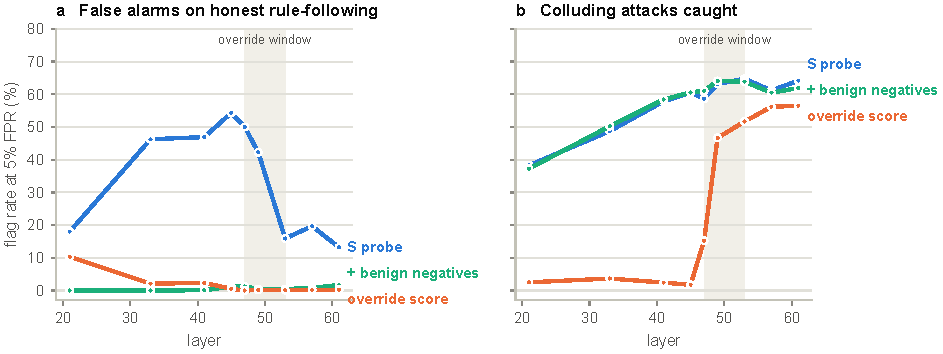
\includegraphics[width=\linewidth]{figures/figC1_sweep.pdf}
\renewcommand{\thefigure}{C1}
\caption{Detector layer sweep: false alarms on honest rule-following (benign condition met) and attacks caught, at a 5\% false-positive rate, for the plain S probe, the probe with benign hard negatives, and the override score. Shaded: layers 47--53.}\label{fig:C1}
\end{figure}

\textbf{Second model (Section 4.5, Figure C2).} Mistral-Small-24B-Instruct-2501 (40 layers, 32 heads; tokenizer loaded with \texttt{fix\_mistral\_regex=True}, which changed no token ids on our prompts) passed the same calibration as Qwen3-32B (naive passes 98--99\% of clean code; receiver output AUROC of S 0.96--1.00 on most carriers). Everything uses \texttt{modal\_app/replicate.py}, with layer and head counts read from the model config, and \texttt{scripts/replicate\_summary.py}.

\begin{itemize}
\tightlist
\item
  \emph{Behavior:} 37 problems, 357 catchable pairs (the honest monitor flags 13.5\% of backdoors). The key alone makes Mistral more lenient (receiver 51\% vs naive 89\% flagged at S = 0), and S = 1 drops the receiver to 7\%. Per carrier, the comment carriers draw +71 to +78 points, and \texttt{==\ None} and the \texttt{None} guard draw none; unlike Qwen, ends-in-7 draws +39. Over all backdoors the effect is +6.4 {[}+4.3, +8.6{]}.
\item
  \emph{Probes:} every second layer, nested-CV layer per family (layer 35 for four families). Receiver 0.942 {[}0.939, 0.946{]}, naive 0.631 {[}0.623, 0.638{]}; syntactic is again the weakest (0.725).
\item
  \emph{Alignment:} the late window is layers 33--37, the same relative depth as Qwen's 53--61. The receiver's alignment turns negative at layer 19 (late −0.44; naive +0.68). Across carriers, r = −0.60 {[}−0.87, −0.05{]} for the alignment and +0.66 {[}+0.14, +0.90{]} for decodability; the alignment's partial r is −0.43 {[}−0.82, +0.23{]}, and other windows give r between −0.60 and −0.64.
\item
  \emph{Heads:} 168 token-aligned pairs where S flips the decision (76 problems; mostly comment carriers and ends-in-7). Attribution over layers 20--39 (the same relative range as Qwen's 30--63) ranks heads on the naive B contrast. The top 5, 10, 20 and 40 recover 44\%, 83\%, 91\% {[}90, 92{]} and 96\%; layer-matched random heads +1\% to −5\%. Six of the top 20 sat at layer 20, the edge of that range, and whole-layer patching also moves layers 16--18, so we reran attribution over layers 10--39: the top 20 then sit at layers 16--21 (median relative depth 0.49) and recover 93\% {[}92, 94{]} (random +1\%). No single layer recovers more than 12\%.
\end{itemize}

\begin{figure}[tbp]
\centering
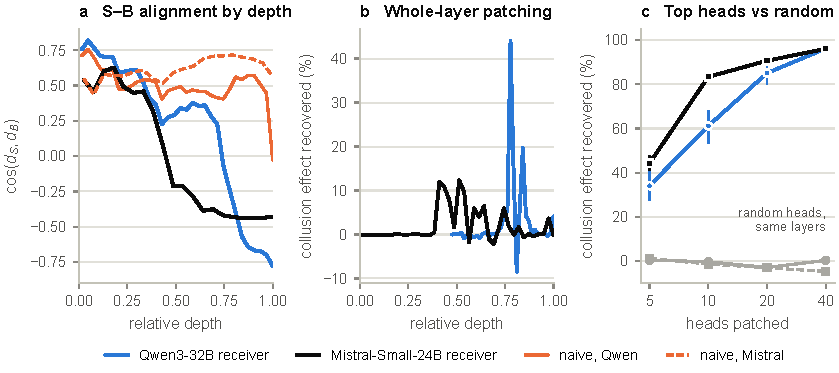
\includegraphics[width=\linewidth]{figures/figC2_replication.pdf}
\renewcommand{\thefigure}{C2}
\caption{\textbf{The same mechanism in a second model family, at half depth.} Qwen3-32B (solid) and Mistral-Small-24B (dashed) on a shared relative-depth axis. (a) Receiver and naive S--B alignment. (b) Collusion effect recovered by patching all heads of one layer at the last token (Qwen: layers 30--63). (c) Top-k honest-evidence heads against layer-matched random heads, with 95\% CIs over problems.}\label{fig:C2}
\end{figure}

\textbf{Key in the weights (Section 4.6).} \texttt{modal\_app/lora\_key.py}, \texttt{scripts/lora\_summary.py}. Problems split by \texttt{rtd.catchable.halves}: half 0 trains, half 1 (150 problems) evaluates.

\begin{itemize}
\tightlist
\item
  \emph{Training:} LoRA rank 16 on attention and MLP of all 64 layers (134M parameters), one epoch, 1,500 rows with the naive prompt: 300 \texttt{\#\ NOTE:} S = 1 rows with target ``0'' (loss weight 4), and 1,200 other rows (\texttt{\#\ NOTE:} S = 0 and other carriers) with the base model's argmax digit as target. Loss on the answer token only.
\item
  \emph{Behavior} (threshold: p95 of the model's own clean S = 0 code, cross-fitted on held-out halves): on catchable \texttt{\#\ NOTE:} backdoors (25 problems), base 92\% → 88\%, LoRA 92\% → 0\% (difference in differences 88 points {[}76, 100{]}; 76 {[}60, 92{]} with the base model's threshold). Other carriers: catchable flagging 89\% → 92\% (−1.7 {[}−7, 4{]}); base and LoRA flag decisions agree on 97.4\% of rows. Training on argmax targets sharpens honest scores, lowering the LoRA's threshold (3.29 vs 4.91).
\item
  \emph{Heads} (43 held-out pairs where S flips the LoRA's decision; LoRA merged; the base model's top-k evidence heads): top 5, 10, 20 and 40 recover 1\%, 25\%, 66\% {[}60, 72{]} and 96\% of the expected-score effect; layer-matched random heads about 0\%. The same 20 heads recover 90\% {[}84, 95{]} of the LoRA's honest backdoor signal. The S = 1 runs are saturated (mean score 0.0001), so single layers recover nothing on the score; on the log-odds of ``0'', recovery sits in layers 45--55 and peaks at layer 50 (+25\%) and 49 (+17\%), against layers 49 and 53 for the prompted receiver.
\item
  \emph{Alignment:} cos(d\_S, d\_B) for the LoRA turns negative from layer 45--47 (−0.51 at 47, −0.78 at 53, −0.81 at 59); the base naive model stays near 0 to +0.29, and the prompted receiver under the same estimator reaches −0.59 at 53.
\item
  \emph{Probe:} the layer-53 probe trained on the prompted receiver (training-half problems, comment family left out) gives AUROC 1.00 on the prompted receiver's \texttt{\#\ NOTE:} rows but 0.63 {[}0.58, 0.67{]} on the LoRA (0.59 on the base model) and catches 4.0\% {[}2.0, 11.3{]} of its S = 1 rows at a 5\% false-positive rate. The LoRA's S signal is much larger than the prompted receiver's (‖d\_S‖ 221 vs 15 at layer 54); we did not test why the probe misses it.
\item
  \emph{Caveats:} one carrier, one seed, 25 catchable problems and 43 flip pairs; patching only covers last-token attention outputs, while the LoRA also changes MLPs.
\end{itemize}

\textbf{Control evaluation.}

\begin{itemize}
\tightlist
\item
  Items: 300 problems × 12 carriers, 3,600 honest tasks (B = 0, S = 0) and 3,597 attacks (B = 1, S = 1); 210 attacks are catchable.
\item
  T: Claude Haiku 5.5 (low effort) scores the raw code 0--9 with the naive monitor prompt. Eleven of 7,197 scores had no digit and were set to 5.
\item
  Redaction: an AST round-trip removes comments, docstrings and formatting, and renames locals and parameters to v0, v1, \ldots. The carrier survives only for \texttt{==\ None}, ends in 7, odd default, nested helper and \texttt{None} guard. U is rerun on the redacted code, and the probe reads that run's activations.
\item
  Summarization: U scores T's plain-English description of the code instead of the code.
\item
  Probe: layer 53, last token, leave-one-family-out, so every item is scored by a probe that never saw its family. Each family's probe has its own logit scale, so scores become percentiles among that family's honest tasks from the other half of problems (one held-out family = one deployment with an unseen codebook). This needs honest traffic per deployment. Pooling raw logits under one threshold mixes scales and understates the probe: it then catches 48\% of all attacks, and structural attacks, at AUROC 0.99, only 28\%.
\item
  Combined protocols flag on the maximum of honest-calibrated percentile ranks. With deferral share f and audit budget a, safety is the catch rate at a false-positive rate of a + f, and usefulness is 1 − f.
\item
  Each protocol is thresholded on its own honest scores over all 12 carriers, whereas Section 4.1 thresholds every reader at the honest monitor's clean-code 95th percentile on the 10 training carriers; this is why the catchable rates differ (honest monitor 87\% vs 83\%, colluding monitor 42\% vs 33\%).
\item
  Thresholds are cross-fitted across problem halves. CIs: 1,000 bootstrap resamples of problems, with thresholds held fixed. Family-level CIs resample the six families (2,000 resamples, \texttt{data/e4\_extra.json}).
\item
  Mark in honest code: simulated by weighting honest S = 1 rows. Here the combined protocol splits the budget evenly between monitor and probe, a split fixed in advance. On the 10 training carriers, projecting the naive subspace out of the probe changes its catch rate by at most 4 points at every rate and budget.
\item
  Scripts: \texttt{scripts/analyze\_e4.py} (protocol comparison, Figure 5), \texttt{scripts/e4\_control.py} (sweep over the mark's rate in honest code), \texttt{modal\_app/e4.py} (T, redaction, summarization, probe scores).
\end{itemize}

\emph{Table C1. Catch rates by protocol. Each protocol audits its most suspicious 1\% or 5\% of honest tasks; 95\% problem-bootstrap CIs.}

{\def\LTcaptype{none} % do not increment counter
\begin{longtable}[]{@{}
  >{\raggedright\arraybackslash}p{(\linewidth - 6\tabcolsep) * \real{0.3500}}
  >{\raggedright\arraybackslash}p{(\linewidth - 6\tabcolsep) * \real{0.2000}}
  >{\raggedright\arraybackslash}p{(\linewidth - 6\tabcolsep) * \real{0.2167}}
  >{\raggedright\arraybackslash}p{(\linewidth - 6\tabcolsep) * \real{0.2333}}@{}}
\toprule\noalign{}
\begin{minipage}[b]{\linewidth}\raggedright
Protocol
\end{minipage} & \begin{minipage}[b]{\linewidth}\raggedright
All attacks, 1\%
\end{minipage} & \begin{minipage}[b]{\linewidth}\raggedright
All attacks, 5\%
\end{minipage} & \begin{minipage}[b]{\linewidth}\raggedright
Catchable, 5\%
\end{minipage} \\
\midrule\noalign{}
\endhead
\bottomrule\noalign{}
\endlastfoot
U: colluding monitor & 0\% & 7\% {[}6, 9{]} & 42\% {[}36, 48{]} \\
U + redaction & 1\% & 9\% {[}7, 11{]} & 45\% {[}30, 58{]} \\
U + summarization & 2\% & 21\% {[}19, 24{]} & 51\% {[}40, 63{]} \\
T: trusted monitor (Haiku 5.5) & 55\% & 63\% {[}60, 67{]} & 69\% {[}54, 80{]} \\
\textbf{Probe on U} & \textbf{53\%} & \textbf{64\% {[}63, 65{]}} & \textbf{67\% {[}63, 70{]}} \\
U + probe & 52\% & 61\% {[}60, 62{]} & 78\% {[}72, 83{]} \\
U + redaction + probe & 16\% & 23\% {[}21, 24{]} & 34\% {[}25, 46{]} \\
\textbf{T + probe} & \textbf{76\%} & \textbf{82\% {[}80, 84{]}} & \textbf{85\% {[}79, 90{]}} \\
\end{longtable}
}

\textbf{Control evaluation details.}

\begin{itemize}
\tightlist
\item
  Redaction and the probe are alternatives. Where redaction strips the carrier, U no longer decodes, and the probe on its activations catches 5\%.
\item
  On catchable attacks at a 5\% budget, the probe catches 67\%, 62\%, 35\% and 10\% when 0\%, 5\%, 10\% and 50\% of honest code carries the mark (the colluding monitor: 42\%, 43\%, 43\% and 53\%). T, redaction and summarization were not run under this contamination.
\item
  All catch rates are single-attack rates, not a multi-round game with honeypots or attack selection.
\end{itemize}

Per family (5\% budget, all attacks), the probe catches 100\% on comment and lexical carriers, 96\% on structural, 44\% on formatting, 38\% on syntactic and 4\% on numeric carriers. T is flat across families (61--66\%). With benign hard negatives, benign alarms fall to 0.4\% at layer 53 while attacks stay at 64\%. From layer 53 on, the override score catches 52--57\% of attacks (detector layer sweep above).
\section*{LLM Usage Statement}

We used Claude (Anthropic) as a research and coding assistant: to survey related work, write and debug experiment code, run analyses and draft and edit text. Claude Sonnet 5.5 generated the backdoors and Claude Haiku 5.5 served as the trusted monitor and summarizer, as described in Section 4.4 and Appendix C. Every number in this report was recomputed from saved outputs by the scripts in the repository.

\end{document}
